\documentclass[11pt]{article}
\usepackage[margin=0.95in]{geometry}
\usepackage{amsmath,amssymb}
\usepackage{graphicx}
\usepackage[hidelinks]{hyperref}
\usepackage{microtype}
\usepackage{booktabs,xcolor}
\definecolor{boxbg}{HTML}{F4F6FA}
\definecolor{rule}{HTML}{2B6CB0}
\newcommand{\entry}[1]{\section*{#1}}
\newenvironment{infobox}{%
  \begin{center}\small\begin{tabular}{@{}l p{0.78\textwidth}@{}}\toprule}%
  {\bottomrule\end{tabular}\end{center}}

\title{\bfseries The Closed Machines of BB(6)\\
\large Nine kernel-checked conditional closures, machine by machine:\\
what each cryptid is, how it was closed, and what remains open}
\author{Enan Srivastava \quad (with an AI assistant; every proof
checked by the Lean 4 kernel)}
\date{September 3, 2026 \quad \texttt{github.com/Enan456/bbchallenge-proofs}}

\begin{document}
\maketitle

\noindent The busy beaver problem at six states is blocked by a
residual set of 1{,}094 machines that defeat every known automated
decider; the community calls them cryptids, because each hides an
iterated arithmetic map of the Collatz kind. This document is a
field guide to the nine that have been \emph{closed}: for each, a
machine-checked theorem states that if one explicit arithmetic
conjecture holds, the machine never halts from the blank tape. Every
theorem is verified by the Lean 4 kernel at the minimal axiom set
$\{\mathrm{propext}, \mathrm{Quot.sound}\}$ with no \texttt{sorry}.
All nine of the program's exact-law machines are now closed.

\begin{center}
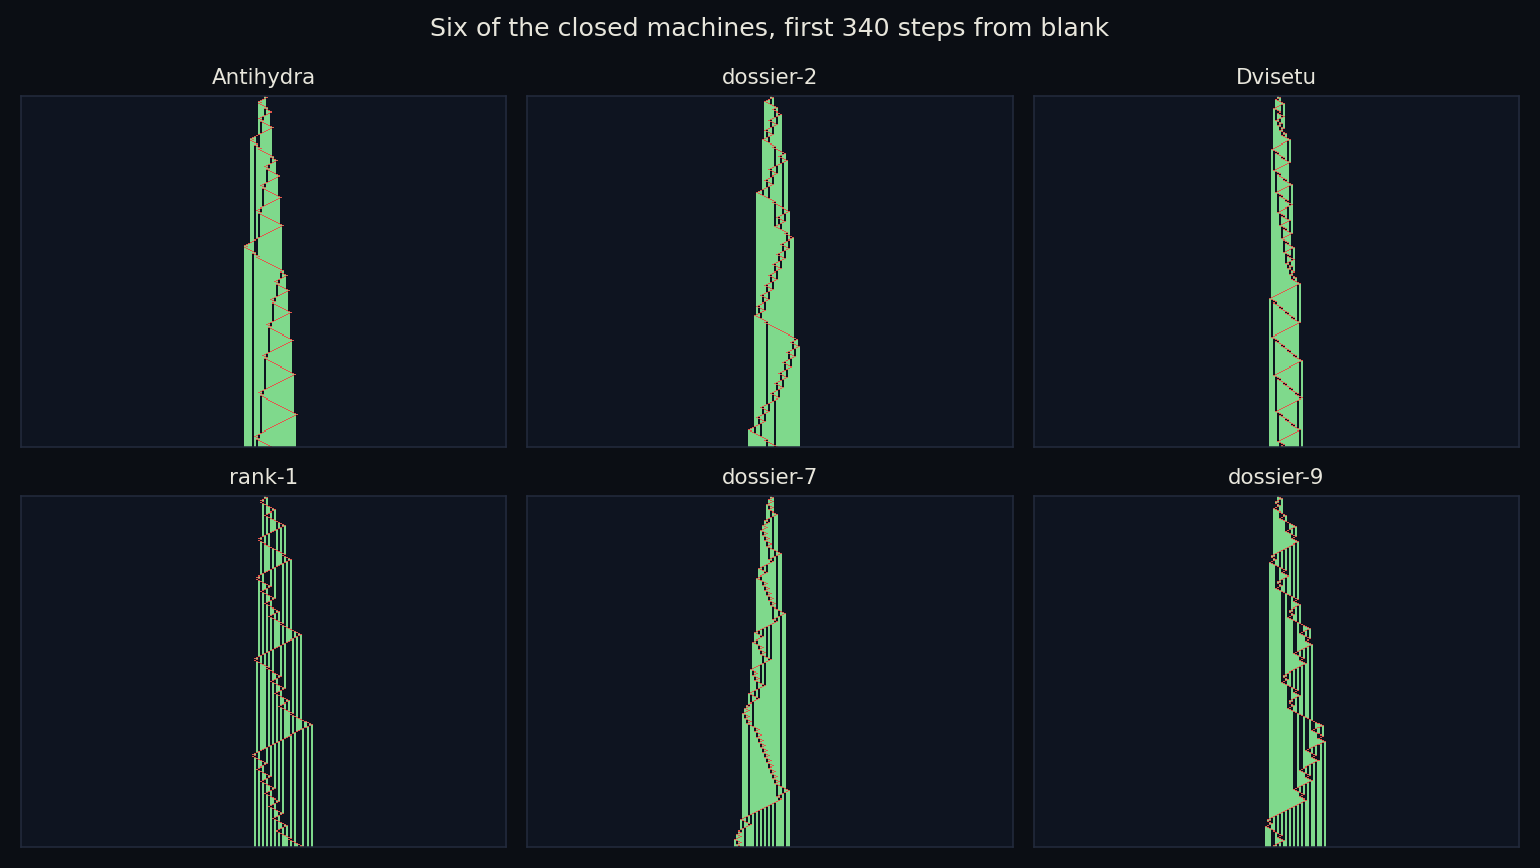
\includegraphics[width=\textwidth]{fig_spacetimes.png}
\end{center}

\section*{The method, common to all nine}

\begin{center}
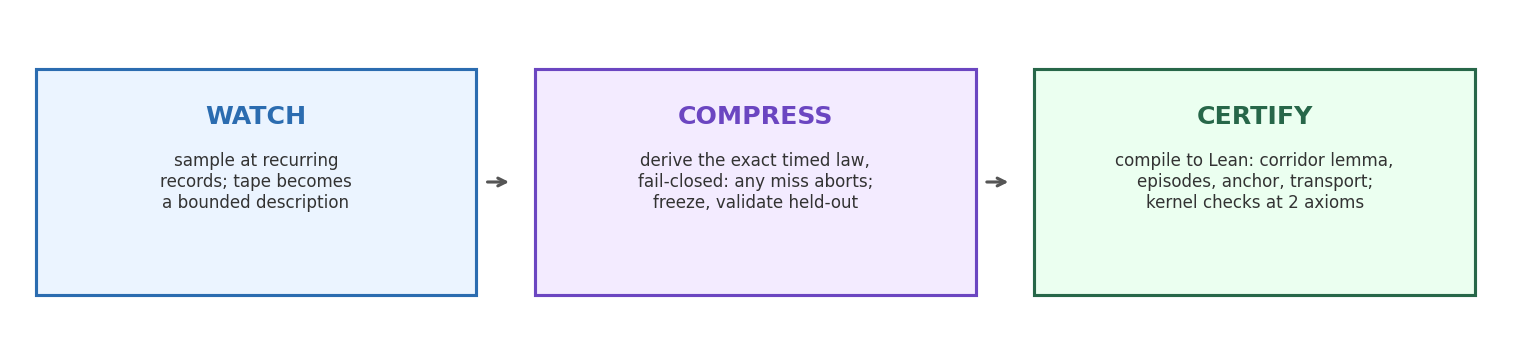
\includegraphics[width=\textwidth]{fig_method.png}
\end{center}

\noindent \textbf{Watch.} Each machine has a natural clock: a
recurring configuration (a record, a spawn entry, an arrival) at
which the tape has a bounded description. Five integers suffice for
dossier-2/3; a triple for Antihydra; one hole and two counters for
Dvisetu; a word of blocks for the rank-1 machine. \textbf{Compress.}
The exact law of that description is derived empirically and
fail-closed: every transition and its exact step count must be
reproduced, and any miss aborts the pipeline. Laws are frozen, then
validated on held-out horizons. \textbf{Certify.} The law is
compiled into Lean: raw semantics; a \emph{corridor lemma} showing
every halt funnels through a single probe pattern; episode theorems
with exact step counts; inductions over the unbounded middles; a
concrete startup anchor; and a transport theorem showing the
abstract orbit predicts the machine forever. The result, per
machine: $\mathsf{Safe} \rightarrow \lnot\mathsf{RawHalts}$, and
(where tested) the sharpness converse: states violating the
conjecture provably halt within tens of steps.

The engineering matured across the closures. The early files
(dossier-2/3, 6{,}000--9{,}000 lines) prove gait-level episodes; the
newest (dossiers 7/8, about 1{,}000 lines each) run their certified
engines at single-raw-step grain, where every branch of the record
law, including residue cases never observed at any empirical
horizon, is simulated exactly with no assumption folded anywhere.

\clearpage
\entry{Antihydra}
\begin{infobox}
code & \texttt{1RB1RA\_0LC1LE\_1LD1LC\_1LA0LB\_1LF1RE\_---0RA} \\
\midrule
status & closed (conditional); the community's best-known cryptid \\
state space & hydra triple $(a, m, c)$; tape $1^a\,0\,1^m\,0\,1^c$ \\
keystone & \texttt{safeOrbitA\_nonhalting} (2{,}130 lines) \\
conjecture & \texttt{SafeOrbitA}: the hydra orbit never dies \\
halt corridor & $F$ entered only via $E0$, moving left \\
validation & mirror exact vs.\ 51.8M raw steps (10{,}001 records) \\
\end{infobox}

\noindent Antihydra iterates a hailstone-like map in which a guard
counter $a$ drifts upward on average while occasional merges spend
it. Death requires the counter to run out, and the walk is a
gambler's ruin with steps $-1/{+}2$ whose ruin probability is the
root of $r^3 - 2r + 1$: exactly $1/\varphi$. The golden ratio
appears in Antihydra's \emph{hazard} where dossier-3 carries it in
its \emph{cone}: same constant, different organs. Two further facts
with closed forms: the realizable dying family $(1,2,c)$ halts in
exactly $(3c^2+44c+125)/4$ raw steps for odd $c$, and the abstract
death cone grows \emph{linearly} (branching constant exactly 1,
backward merges throttled by the $a \ge 2$ guard), the third data
point in the program's branching-constant series
$\{\varphi,\ \text{2-adic},\ 1\}$.

\begin{center}
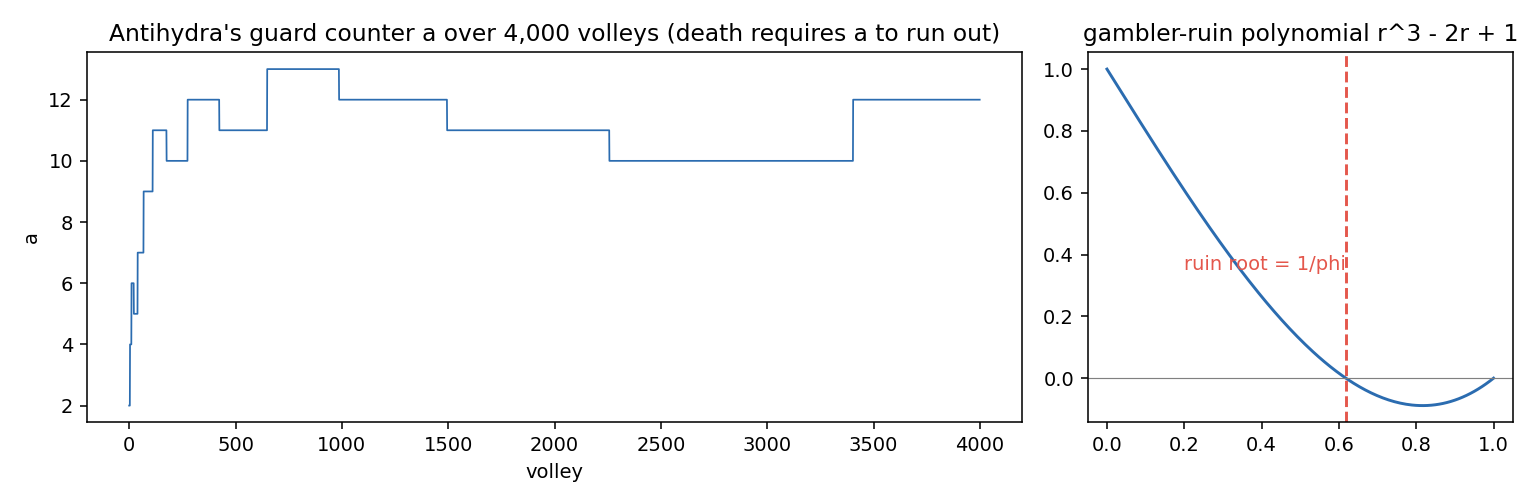
\includegraphics[width=\textwidth]{fig_antihydra.png}
\end{center}

\entry{Dossier-1}
\begin{infobox}
code & \texttt{1RB0LE\_1LB1RC\_0RF0RD\_1RE0LA\_1LA1RE\_---0RB} \\
\midrule
status & closed (conditional) \\
state space & a stack of levels (chain orbit) \\
keystone & \texttt{dossier1\_nonhalting} (5{,}770 lines) \\
conjecture & the abstract chain orbit never dies \\
halt corridor & \texttt{halt\_requires\_c\_probe\_00} \\
\end{infobox}

\noindent The program's first original closure and the template for
everything after it: the layered endgame (halt localization, then an
invariant discharged by a raw-to-macro closure induction) that later
files industrialized. Its 33 macro obligations were first discharged
empirically at $10^8$ steps, then certified.

\clearpage
\entry{Dossier-2 and dossier-3 (the mirror pair)}
\begin{infobox}
codes & \texttt{1RB1RC\_1LC1LC\_1RE0LD\_1LB1RF\_---1RA\_0RD1RD} \newline
        \texttt{1RB1RB\_1LC0RE\_---1LD\_0RA1LB\_1RA1LF\_0LE1LE} \\
\midrule
status & closed (conditional); one law, two machines \\
state space & five integers: block ends $l, r$, holes $h_1, h_2$, tag \\
keystones & \texttt{dossier2\_nonhalting} (6{,}130 lines),
\texttt{dossier3\_nonhalting} (9{,}020) \\
conjecture & \texttt{SafeMetaOrbit}: the five-integer iteration
never enters an explicit fatal set \\
halt corridor & the probe event: $C$ reads 0 with a 0 to its right \\
validation & predictor exact over $10^9$ raw steps per machine;
seven episode theorems with exact step counts (crawl 10, cross 13,
terminate 13, fuse 19, \ldots) \\
\end{infobox}

\noindent The flagship reduction. At every spawn entry the tape is a
solid block of 1s with exactly two holes; seven certified episodes
cover everything the machine does. Sampling at renewals collapses
the dynamics to a closed-form two-counter map whose fatal set is a
width-five window around the diagonal; the orbit avoids it for
$10^8$ iterations (about $10^{15}$ raw steps) with minimum margin 4.
The proof routes that fail are themselves mapped: no congruence
invariant to modulus 384, factor complexity $\sim 1.6^n$ (not a
rotation), and 33{,}551 ranking-class halfplane families
exhaustively refuted on the true fatal model. Dossier-3's abstract
death cone is an exact Fibonacci tree ($L(k)=L(k{-}1)+L(k{-}2)$,
branching at $\varphi$, mechanism: no terminate follows terminate).

\begin{center}
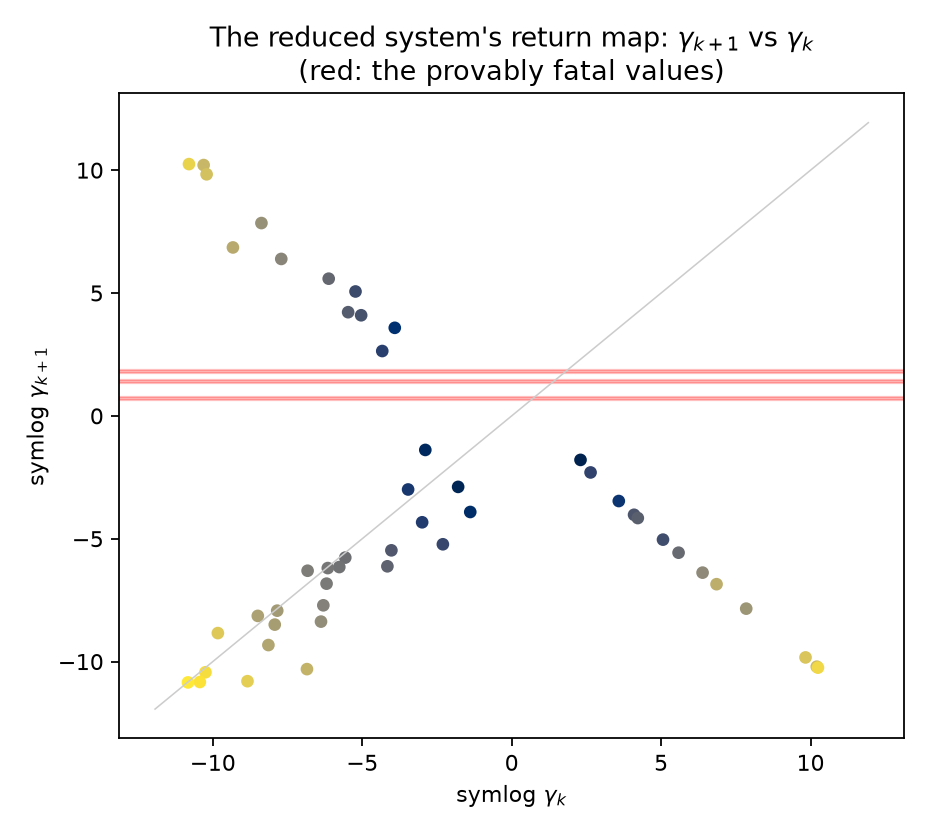
\includegraphics[width=0.62\textwidth]{fig8_returnmap.png}
\end{center}

\clearpage
\entry{Dvisetu (dossier-6)}
\begin{infobox}
code & \texttt{1RB0RB\_1LB0LC\_1RD1LC\_1RE0RA\_0RF1RA\_---1LB} \\
\midrule
status & closed (conditional); this program's own miner candidate
(July 2026), re-surfaced blind by the deep sweep \\
state space & one hole, two counters: $1^a\,0\,1^b$, plus
checkpoint scalars $1^n$ \\
keystone & \texttt{safeDvisetuOrbit\_nonhalting} (1{,}942 lines) \\
conjecture & \texttt{SafeCheckpointOrbit} (orbit guards $+$ the
divide episode, folded as \texttt{DivideFaithful}) \\
halt corridor & $E$ reading 0 with a 0 to its \emph{right} \\
validation & 2{,}746/2{,}746 timed record transitions at
$2\times10^7$ steps; divide sub-rule 5/5 to $n = 18{,}648$ \\
\end{infobox}

\noindent The simplest state geometry in the program, and a genuine
generalized-Collatz specimen: drift $(a,b) \to (a{+}4, b{-}3)$ at
exactly $(32b-41)/3$ steps per record, collapse to a single block,
then a renewal branched on $n \bmod 3$, whose $n \equiv 0$ branch
\emph{divides by} 3 recursively (divide while the quotient is
$0 \bmod 9$, base case by the residue mod 9). The drift gait
resolved into four passes over a five-step motif, making the step
count integral by construction. From dossier opening to
kernel-checked closure: about 36 hours.

\begin{center}
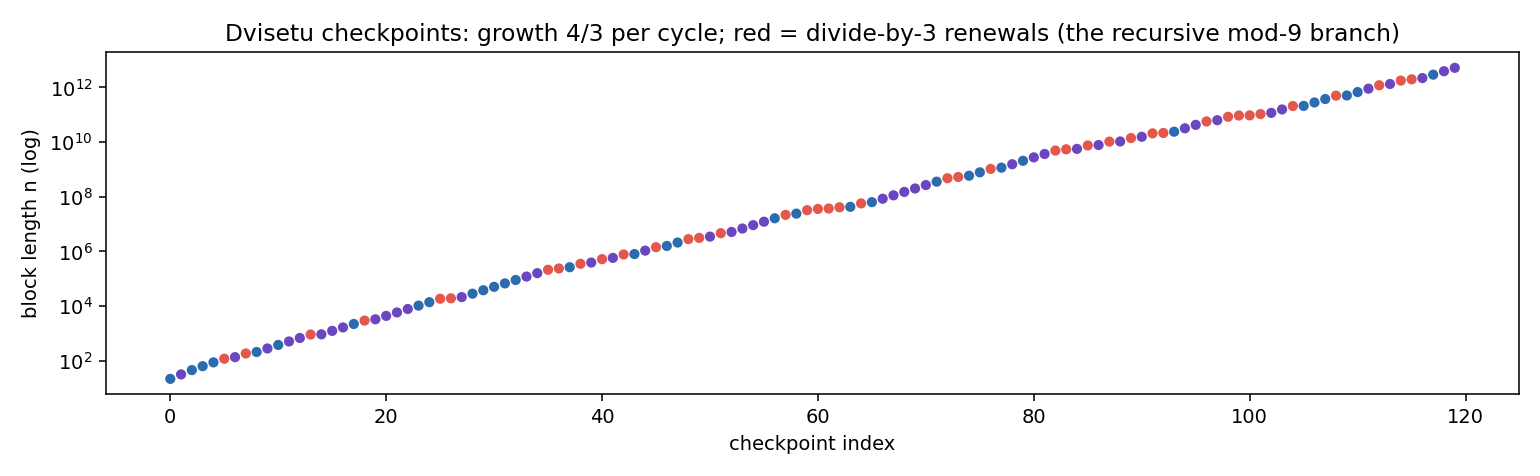
\includegraphics[width=\textwidth]{fig_dvisetu.png}
\end{center}

\entry{Rank-1 (dossier-5): the first growing-dimension closure}
\begin{infobox}
code & \texttt{1RB1RD\_1LC0LC\_0RD0LB\_1RF0LE\_0RD---\_0RA1RC} \\
\midrule
status & closed (conditional); first closure on a state space of
growing dimension \\
state space & a \emph{word} of 1-blocks (lengths 1/2/3, single-0
gaps) that grows without bound \\
keystone & \texttt{safeWordOrbit\_nonhalting} (2{,}126 lines),
zero folded assumptions \\
conjecture & \texttt{SafeWordOrbit}: the word orbit never dies
(a single clause) \\
halt corridor & $D$ reads 1 with a 1 to its left \\
validation & calculus frozen-exact 2{,}179/2{,}186 at
$2\times10^8$ steps; reseed differentials exact; Lean mirror
realizes every arrival configuration at the predicted cumulative
time over 2.2M steps \\
\end{infobox}

\noindent Semantically a two-phase odometer on $\{1,3\}$-words: the
3-blocks are carries traveling in wave trains, a deposited 2-block
is a cursor that restarts the next pass at its own position, and the
boundary rule is a literal block trisection $3 \mapsto 1,1,1$. Its
death tree branches 2-adically in train lengths (the number of
one-sweep preimages of a word is exactly $\prod_i
2^{\max(0,t_i-2)}$), where dossier-3's branches at $\varphi$. The
certified layer works at cell grain, one level below the learned
calculus, where the boundary families and the decision function are
subsumed and proven.

\begin{center}
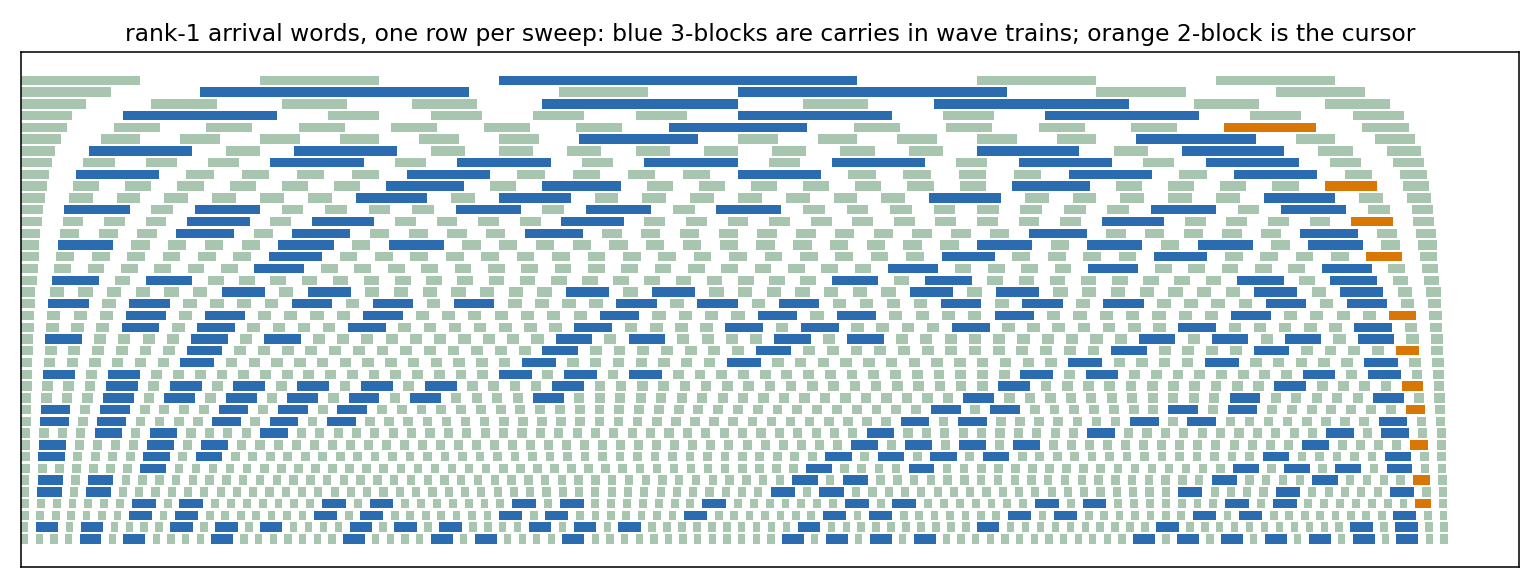
\includegraphics[width=\textwidth]{fig_rank1.png}
\end{center}

\clearpage
\entry{Dossiers 7 and 8: the raw-step-grain pair}
\begin{infobox}
codes & \texttt{1RB1LA\_1LC0RE\_1LF1LD\_1RE0LC\_1LB1RA\_---0LA} \newline
        \texttt{1RB0LC\_1LC0RD\_1LF1LA\_1LB1RE\_1RB1LE\_---0LE} \\
\midrule
status & closed (conditional); the strongest engineering of the set \\
state space & unary-ladder words $1^a\,0\,1\,0\,1^b\,0\,(1\,0)^k
\cdots$ growing left; counters $(a,b,k)$ and $(a,b,k,g)$ \\
keystones & \texttt{safeD7Orbit\_nonhalting} (1{,}036 lines),
\texttt{safeD8Orbit\_nonhalting} (1{,}037) \\
conjecture & the word orbit never dies (single clause each) \\
halt corridor & $F$ entered only from $C0$; probe: $C$ reads 0
needing a 1-guard to its left \\
validation & design mirrors 5{,}263/5{,}263 and 3{,}890/3{,}890
record transitions at $2\times10^7$ steps, validated before any
Lean was written; 20{,}000 randomized episode plants each \\
\end{infobox}

\noindent Sibling machines with opposite ladder parity (and, for
dossier-8, an epoch counter). Their certified engines run at
single-raw-step grain: every raw move is one of three proven
episodes on a boundary pair, so \emph{every} branch of the 13- and
12-rule record laws, including residue cases whose first occurrence
is projected near $3\times10^{12}$ steps, is simulated exactly and
proven faithful. Nothing is folded; the only fail-closed exits are
the genuine halt patterns and fuel.

\begin{center}
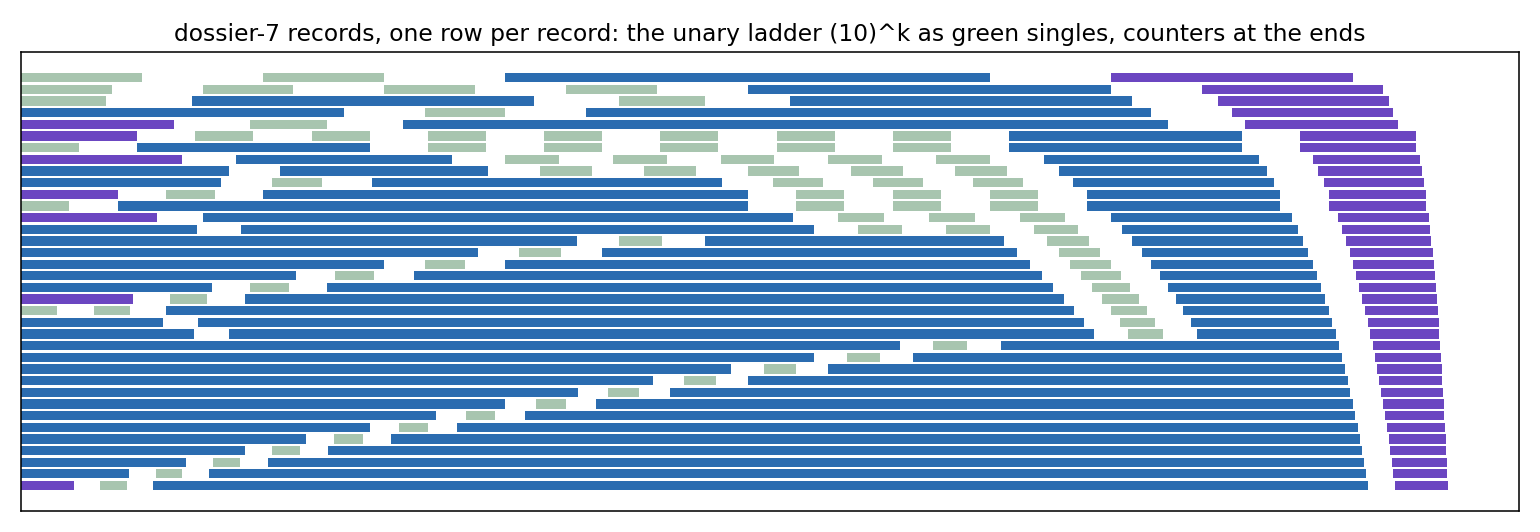
\includegraphics[width=\textwidth]{fig_d7.png}
\end{center}

\entry{Dossier-9}
\begin{infobox}
code & \texttt{1RB0LF\_1RC---\_1LD0RF\_1RA0LE\_0LD1LD\_0RD0RB} \\
\midrule
status & closed (conditional); the ninth and final exact-law machine \\
state space & words on a right-growing frontier; parametric calculus
at 100.00\% held-out (271{,}344/271{,}344 segments at $8\times10^6$
steps) preceded the closure \\
keystone & \texttt{safeD9Orbit\_nonhalting} (1{,}059 lines),
single-raw-step engine, zero folds \\
conjecture & \texttt{SafeD9Orbit}: the word orbit never dies \\
halt corridor & the simplest of the set: the fatal probe \emph{is}
the halt ($B$ reads 1; $B$ entered only via $A0$ or $F1$) \\
validation & mirror 5{,}804/5{,}804 record transitions exact at
$2\times10^7$ steps; fuel margin 2{,}039$\times$; 20{,}000
randomized episode plants \\
\end{infobox}

\clearpage
\clearpage
\section*{Anatomy of a closure: the seven layers}

Every closure file, from dossier-2's 6{,}130 lines to dossier-9's
1{,}059, is the same proof in seven layers. What changed across the
program is only the \emph{grain} at which layer four is built.

\paragraph{1. Raw semantics.} The machine table as an inductive
definition, one-step and $n$-step relations, and \texttt{RawHalts}.
Nothing imported beyond Lean core: the files are self-contained down
to the kernel.

\paragraph{2. Halt localization (the corridor lemma).} Each machine
has exactly one undefined transition, and working backward through
the table funnels every halt through a single \emph{probe pattern}.
Verbatim from Dvisetu:
\begin{small}
\begin{verbatim}
theorem halt_requires_e_probe_00 {c : Config} (hne : c.state <> State.F)
    (hh : RawHalts c) :
    exists d, Reaches c d /\ d.state = State.E /\
      d.tape d.head = false /\ d.tape (d.head + 1) = false
\end{verbatim}
\end{small}
Everything downstream reduces to: the probe never fires. Dossier-9's
corridor is the degenerate ideal, where the probe \emph{is} the halt
and safety is a one-cell predicate.

\paragraph{3. Probe safety as an invariant over segments.} A
predicate (\texttt{EProbeSafe}, \texttt{DProbeSafe},
\texttt{BProbeSafe}, per machine) plus segment-induction machinery:
if every certified episode preserves safety and covers the run, the
probe never fires between anchors.

\paragraph{4. Episode theorems: the certified choreography.} The
heart of each file, and where the behaviour of the machine lives.
An episode theorem states: from any configuration matching a shape
(given by parameters), the machine runs an \emph{exact} number of
steps, produces an \emph{exact} output shape, and is probe-safe
throughout. Verbatim from Dvisetu's drift:
\begin{small}
\begin{verbatim}
theorem drift_step {cfg : Config} {g : Int} (n : Nat) (hn : 1 <= n)
    (hs : cfg.state = State.B) (hh : cfg.head = g + 3 * n + 2)
    (hgap : cfg.tape g = false)
    (hones : forall i, i < 3 * n + 1 -> cfg.tape (g + 1 + i) = true) : ...
\end{verbatim}
\end{small}
The statement quantifies over the unbounded parameter ($n$, with
$b = 3n+1$), so one theorem covers infinitely many raw-step runs;
the proof is an induction whose base and step are bounded
evaluations. This is the compression that lets verification outrun
the machine.

\paragraph{5. The startup anchor.} From the blank tape to the first
abstract state, certified step by step (235 concrete steps for
dossier-2; Dvisetu's is 6; dossiers 7--9 use a \emph{virtual anchor},
the blank tape itself realizing the empty word, so no prefix at all).

\paragraph{6. The abstract orbit and transport.} An executable step
function on the abstract state (five integers, a checkpoint scalar,
a word), iterated from the anchor; a \texttt{Realizes} grammar tying
abstract states to literal tapes; and the transport theorem: if the
abstract step yields a successor, the raw machine, started on any
realization, reaches a realization of that successor in exactly the
predicted number of steps, safely. Verbatim from dossier-7's engine:
\begin{small}
\begin{verbatim}
def wfuel (w : List Bool) : Nat := 64 * (w.length + 64) * (w.length + 64)
def wstep (st : State) (w : List Bool) : Option (State x List Bool x Nat)
-- "The sweep is faithful": whenever wstep yields a successor arrival,
-- the raw machine, started on any realization of the input, ...
\end{verbatim}
\end{small}

\paragraph{7. The keystone.} \texttt{Safe} says the abstract orbit
never returns \texttt{none}; the keystone composes layers 2--6 into
$\mathsf{Safe} \rightarrow \lnot\mathsf{RawHalts}$. The kernel then
replays the whole file; the build itself prints the axiom report.

\section*{The grain ladder: three ways to build layer four}

\textbf{Gait grain} (dossiers 1--3, Antihydra, Dvisetu): episodes are
the machine's natural gaits, discovered by instrumentation (dossier-2
walks in a fixed ten-step crawl; Dvisetu's drift is four passes over
a five-step motif). Maximal legibility: the certified objects are
recognizably \emph{behaviours}, and their exact step counts
($10$ per crawl cycle, $(32b-41)/3$ per drift record) become theorem
constants. Cost: every boundary case needs its own episode, and a
genuinely hard one (Dvisetu's divide renewal) must either be proven
or folded into the conjecture as a named assumption.

\textbf{Cell grain} (rank-1): episodes are bounded-window
micro-moves, one level below the learned calculus. The boundary
families and even the decision function of the word calculus turn
out to be \emph{consequences} at this grain, so nothing is folded.
The certified layer no longer mentions trisection or cursors by
name; the conjecture absorbs the law, and the law's legibility lives
in the (validated, untrusted) empirical layer.

\textbf{Raw-step grain} (dossiers 7--9): the terminus. Every raw
move is one of three proven episodes on a boundary pair; a
fail-closed sweep with quadratic fuel runs record to record. Every
branch of the record law, including residue cases first occurring
near $3\times10^{12}$ steps, is simulated exactly; the only
\texttt{none} exits are the genuine halt patterns and fuel. Files
shrink to $\sim$1{,}000 lines. The trade: the conjecture is about an
orbit the file computes but does not explain; the \emph{explanation}
(drift laws, ladders, renewals) stays in the empirical layer, which
is where the mathematics of the conjecture gets done anyway.

The progression is not merely stylistic. Gait grain proves the most
\emph{about} the machine; raw-step grain proves the most
\emph{coverage} for the least trust surface. The program now holds
both ends, and the right choice per machine is: gait grain where the
conjecture will be attacked analytically (dossier-2/3's renewal map
feeds the invariant-measure program), raw-step grain where closure
and external checkability are the goal.

\section*{The trust chain, stated exactly}

\emph{Trusted}: the Lean kernel, \textsf{propext},
\textsf{Quot.sound}, and the machine table transcribed in layer 1.
Nothing else. \emph{Untrusted but validated}: everything that found
the proofs -- the finders, segmenters, calculus learners, the python
mirrors, the AI that drafted the Lean. Their role is discovery; a
wrong law would simply have failed to compile into theorems, and a
wrong mirror is caught by the differential tests
(\texttt{tests/bb6/test\_*\_theorems.py}: randomized episode plants
checked cell-for-cell with exact step counts and probe ledgers, plus
the abstract mirror replayed against millions of raw steps). The
fail-closed discipline runs through every layer: learners abort on
unexplained events, \texttt{wstep} returns \texttt{none} rather than
guess, and the conjectures quantify over exactly the executable
orbit, so there is no gap between what is conjectured and what is
computed.

\section*{The certified behaviours, as a bestiary}

What the nine closures actually pin down, machine by machine, is a
small zoo of arithmetic behaviours:

\begin{itemize}
\item \textbf{Drift-and-renewal two-counter maps} (dossier-2/3
reduced form; Dvisetu at checkpoint level): a counter drains
linearly while another grows, then a renewal reseeds by subtraction,
swap, or division, with parity or residue choosing the branch. Death
is a near-tie or a residue window; the orbits graze it (margin 4 for
dossier-2/3) and survive.
\item \textbf{Guarded random walks} (Antihydra): a counter with
drift $+0.47$ per volley whose death is gambler's ruin at
$1/\varphi$; deaths are early-game and confined to a bounded slab.
\item \textbf{Odometers on words} (rank-1): carries as 3-blocks in
wave trains, a cursor as the carry boundary, block trisection at the
frontier; preimage multiplicity exactly $\prod 2^{\max(0,t_i-2)}$.
\item \textbf{Unary-ladder counters} (dossiers 7--8): a $(10)^k$
ladder drained and reloaded by minor and grand renewals at growth
$\sim 3/2$; the state is a fixed integer vector wearing an
unbounded unary coat.
\item \textbf{Lethality, measured and proven}: the closures are
sharp. Danger-band states of dossier-2 halt in 6--12 raw steps when
materialized; Antihydra's dying family halts in exactly
$(3c^2+44c+125)/4$ steps; 20{,}000 random hole-perturbations of live
states produce zero halts. The conjectures are equivalences in
practice: leaving the safe region is not unproven-safe, it is fatal.
\item \textbf{The backward view}: death cones with per-machine
branching constants ($\varphi$, 2-adic, exactly 1), each traceable
to an alternation constraint; every record configuration provably
$\ge 24$--$30$ raw steps from any halt.
\end{itemize}

\section*{What the conjectures have in common, and what remains}

Every closure ends at a Collatz-class orbit-avoidance statement, and
the program has mapped why no shortcut exists: a sound invariant
search over every learned law in the cohort (congruence closures to
modulus 64, monotone functionals, two independent implementations
that first cross-audited each other) found \emph{zero}
invariant-decidable machines, and ranking-class certificates were
exhaustively refuted on the one system with a complete fatal model.
The orbits avoid death for measure-theoretic reasons (drift,
uniform hazard, Borel--Cantelli tails, seed-space density
$\approx 12/X$), and finite certificates cannot see
measure-theoretic truths. The standing deep project is the
invariant-measure route: the renewal maps here are explicit, total,
and piecewise affine with verified uniform hazard, materially
better conditioned than Collatz itself.

\section*{Verify everything yourself}

\begin{verbatim}
git clone https://github.com/Enan456/bbchallenge-proofs
cd bbchallenge-proofs/busy-beaver-core && lake build
# the build prints, per keystone theorem:
#   depends on axioms: [propext, Quot.sound]
\end{verbatim}

\noindent External approval path: Palomar registration (entries
pinned and validated; one browser session), bbchallenge forum
publication with invited reproduction (post drafted), and DeepMath
2026 review (extended abstract at v19). No process makes these
unconditional; approval means externally re-verified reductions,
each machine's halting problem restated as one explicit arithmetic
question.

\end{document}
